%    Template for seminar reports
% Seminar Current Topics in Computer Vision and Machine Learning
% Summer Semester 2015
% Computer Vision Group, Visual Computing Institute, RWTH Aachen

\documentclass[twoside,a4paper,article]{combine}


% =========================================================================
\usepackage[utf8]{inputenc}
%\usepackage[ngerman]{babel}
\usepackage{a4}
\usepackage{fancyhdr}   
%\usepackage{german}    % Uncomment this iff you're writing the report in German
\usepackage{makeidx}
\usepackage{color}
\usepackage{t1enc}		% german letters in the "\hyphenation" - command
\usepackage{latexsym}	% math symbols
\usepackage{amssymb}    % AMS symbol fonts for LaTeX.
\usepackage{amsmath}

\usepackage{graphicx}
\usepackage{pslatex}
\usepackage{ifthen}

\usepackage[T1]{fontenc}
\usepackage{pslatex}

\usepackage{psfrag}
\usepackage{subfigure}
\usepackage{wrapfig}
\usepackage{url}

% =========================================================================

\setlength{\oddsidemargin}{3.6pt}
\setlength{\evensidemargin}{22.6pt}
\setlength{\textwidth}{426.8pt}
\setlength{\textheight}{654.4pt}
\setlength{\headsep}{18pt}
\setlength{\headheight}{15pt}
\setlength{\topmargin}{-41.7pt}
\setlength{\topskip}{10pt}
\setlength{\footskip}{42pt}

\setlength{\parindent}{0pt}

% =========================================================================

\graphicspath{
	{img/}
}

%%%
% We want also subsubsections to be enumerated
%%%
\setcounter{secnumdepth}{3}
\setcounter{tocdepth}{3}

\makeglossary
%\makeindex

% =========================================================================
\begin{document}

% Template for seminar reports
% Seminar Current Topics in Computer Vision and Machine Learning

\begin{titlepage}


\begin{center}
\ 
\vspace{3.5cm}


\textsf
{
Fakultät für Mathematik, Informatik und Naturwissenschaften\\
Lehr- und Forschungsgebiet Informatik VIII\\
Computer Vision\\
Prof. Dr. Bastian Leibe
}

\rule{\linewidth}{1pt}

\vspace{1.75cm}
\LARGE
\textbf{Seminar Report}

\vspace{1.7cm}
\huge
Combining 3D Shape, Color, and Motion for Robust Anytime Tracking

\vspace{3.0cm}
\Large
Frederik Zwilling\\
\large
Matriculation Number: 304314

\vspace{0.5cm}
June 2015

\vspace{1.05cm}
\rule{\linewidth}{1pt}

\vspace{0.5cm}
\textsf{\textbf{
\normalsize
\begin{tabular}{ll}
Advisor:  & Aljoša Ošep\\
\end{tabular}
}}
\end{center}

\end{titlepage}


\begin{abstract}
  \textcolor{red}{Abstract}
\end{abstract}

\tableofcontents
\newpage
% =========================================================================

\section{Introduction}
\label{sec:intro}
Robust and precise position and velocity estimation is an important
part of object tracking. It is an essential part in the collision
avoidance of an autonomous car, for example. This report presents a
method by Held, Levinson, Thrun, and Savarese to solve this part of
the tracking problem by combining the 3D shape, color and motion of
the tracked object~\cite{paper}. The method uses a probabilistic
measurement model in form of a Dynamic Bayesian Network. The state
space of position and velocity for each tracked object is represented
in a special dynamic histogram, called \textit{annealed dynamic
  histogram}. This histogram dynamically increases its resolution in
the important areas and considers the local resolution in the
measurement model. By expanding the measurement model with color the
method results can be further improved. This is shown by the authors
by evaluating in a static environment where only the reference system
is moving and in a dynamic environment where the compactness of the
models build with the tracking results is used as evaluation criteria. 


\subsection{Motivation}
\label{sub:motivation}
Robotic applications are about to change many domains from the ground
up. Especially autonomous systems could take over dangerous,
exhausting and unpopular tasks and allow humans to do more satisfying
tasks instead. Additionally, autonomous systems can be more efficient
and scalable than solving the tasks by hand. Some progressive domains
with autonomous robots are flying drones, which can map
areas~\cite{auto-drones} or deliver
packages~\cite{auto-delivery-drones}, autonomous cars, which take care
of driving~\cite{auto-cars}, logistic robots, which store and grab
goods in warehouses~\cite{kiva}, and domestic service robots, which
can support old people and clean at home~\cite{athome}. All these
domains have in common that the robots have to track objects in their
environment, mostly for avoiding collisions, in the case of domestic
service robot also to follow people for example. Often the reliability
and precision of the tracking are limiting factors. An autonomous car,
for example, can only drive fast if it is absolutely sure that it
tracks all objects in the surrounding correctly and none of these
objects could cause a collision.  This report mainly focuses on the
domain of autonomous cars. Here, the autonomous system takes care of
the time consuming driving task on the one hand and could help to
reduce the amount of traffic deaths ($25,938$ in $2013$ in the
EU~\cite{traffic-deaths}) on the other hand. In this domain it is
especially important to estimate the speed of various nearby objects
robustly and in real time. Figure~\ref{fig:objects} shows the three
main classes of objects that have to be tracked, cars, bicycles, and
pedestrians, in challenging situations. The method proposed in this
report solves this task and performs better than previous approaches
in the car domain.
\begin{figure}
  \subfigure[Cars on a highway]{%
    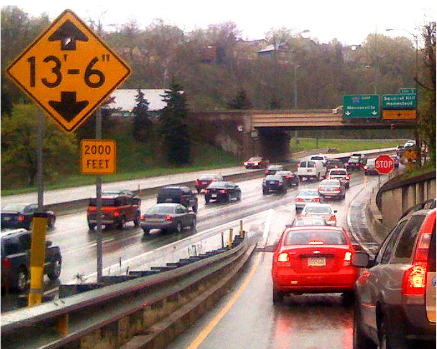
\includegraphics[height=.3\linewidth]{highway}
  }
  \subfigure[A cyclist]{%
    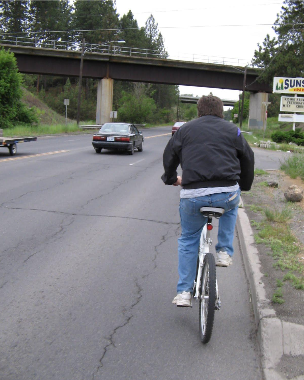
\includegraphics[height=.3\linewidth]{bicycle}
  }
  \subfigure[A pedestrian]{%
    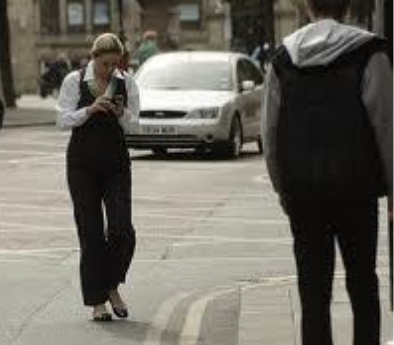
\includegraphics[height=.3\linewidth]{pedestrian}
  }
  
  \caption{Various objects that have to be tracked in challenging
    situations~\cite{held-website}}
  \label{fig:objects}
\end{figure}


\subsection{Tracking}
\label{sub:tracking}
Object tracking is the complex task to identify objects and their
movement over time. It can be separated into the following parts. The
first step segments the sensor data for time $t$, called
\textit{frame}, into detected objects. This can be done for example by
separating foreground and background and find connected components in
the foreground. In this step it is beneficial to use that
the most important objects to find are cars, bicycles and
pedestrians~\cite{segmentation}. The second step is to associate
detected object in the successive frames $t$ and $t+1$. One method to
find these matchings is to compute descriptors, such as the HOG
descriptor, for the objects and find nearest neighbors in the
descriptor space~\cite{arbitrary-object-recognition}. The third step
is the position and velocity estimation of the tracked object. That is
the part of tracking this report is about.

The data that is used for tracking in this report is generated by a
dense laser sensor that measures the distance to surrounding objects
with multiple rotating laser beams. Such a sensor and the data
generated by it is shown in Figure~\ref{fig:lidar}. Additionally, the
sensor provides a camera image similar to a panorama.
\begin{figure}
  \center
  \subfigure[]{%
    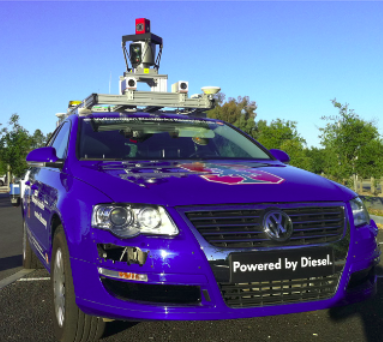
\includegraphics[height=.35\linewidth]{lidar}
  }
  \subfigure[]{%
    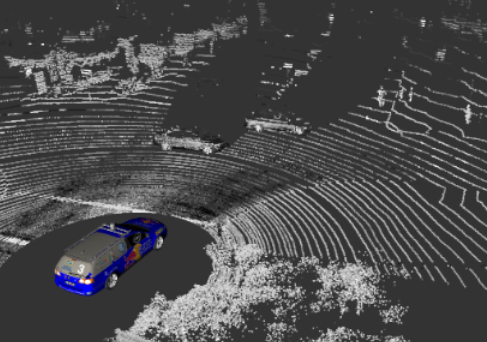
\includegraphics[height=.35\linewidth]{lidar-data}
  }
  
  \caption{A Velodyne LIDAR sensor mounted on a car (a) and a
    visualization of the point cloud generated by it
    (b)~\cite{arbitrary-object-recognition}.}
  \label{fig:lidar}
\end{figure}

\subsection{Velocity and Pose Estimation}
\label{sub:vel-and-pos-estimation}
To compute the pose and velocity estimation of an object, we first
introduce a measurement model that is derived from a Dynamic Bayesian
Network (\textit{DBN}). This DBN models for each frame the
dependencies between position, velocity, object surface and the
observed measurement as well as the dependencies between two
frames. This model uses shape and motion. Though tracking is a hard
problem because in cases with occlusion and major changes in the
viewpoint the visible object surface can differ significantly and
introduce an error. Especially in these cases, it is intuitive to also
consider color in the measurement model because the additional
information is influenced less by occlusion and viewpoint changes.

To find the state, which is composed of position and velocity of an
object, we use a histogram that maps the each histogram-chunk in the
state space to the probability that this chunk causes the measurement
according to our model. This allows a global search in the state space
with multiple hypothesis. A standard histogram with adequate
resolution would have to many chunks and thus would be to slow for
real time computation. Therefore, we use a dynamic histogram that
starts with a low resolution and an approximated posterior
distribution. Then it dynamically increases the resolution in areas
with high probability to cause the measurement. This allows to achieve
a result after running the method for any time. The downside of the
dynamic histogram is that the initial low resolution introduces an
additional error. This can be balanced by including the resolution in
the measurement model. We call this method \textit{annealed dynamic
  histogram} because as the resolution increases, the distribution is
annealed and approaches the true posterior.

The evaluation in Section~\ref{sec:evaluation} shows that the method
outperforms other tracking methods by about $10\%$.
\textcolor{red}{Maybe add more evaluation intro?}

% +++++++++++++++++++++++++
\section{Related Work}
\label{sec:related-work}
The tracking problem has been studied for many years. The most common
approaches to estimate the position and velocity of tracked objects,
namely Kalman filters and Iterative Closest Point,
are described in subsection~\ref{sub:pos-vel-est-alt}. Often these
approaches are efficient but sacrifice a lot of the available data by
using simple representations or search only for a local maximum.
Because
our case of tracking objects in 3D point clouds from a laser sensor is
only a special case of tracking,
subsection~\ref{sub:slternative-sensors} gives an overview of the
tracking approaches with other sensors, mainly single cameras and
stereo cameras.
Subsection~\ref{sub:grid-based-methods} presents
grid-based approaches that are similar to annealed dynamic histograms.

\subsection{Position and velocity estimation alternatives}
\label{sub:pos-vel-est-alt}
A simple approach to estimate position and velocity of a tracked
object first represent the object by its
centroid~\cite{kalman-centroid, towards-aut-cars} or bounding
box~\cite{kalman-bounding-box, kalman-bounding-box2,
  kalman-bounding-box3} and then use a Kalman
filter~\cite{ai-modern}. This is a computationally efficient approach
but discards a lot of available information by using such a simple
representation. Therefore this approach is especially fragile in cases
of occlusion and viewpoint changes. In the occlusion case, the
bounding box can contain only a part of the object and the centroid
would be shifted. In the viewpoint-change case the centroid and
bounding box can significantly differ (e.g. when seeing a cyclist from
the back and the side). Another disadvantage of the Kalman filter is
that it can only represent a single hypothesis and thus performs
poorly when multiple hypotheses are reasonable.

Other approaches include domain specific knowledge to use better
fitting object representations. For example the typical shape of a car
with its corners or wheels could be use to achieve a more precise
position of an object in a frame~\cite{use-car-shape, use-car-shape2,
  use-car-shape3}. This provides better detection and association
results but is limited by the amount of trained
object-classes. Although cars, pedestrians and cyclists are the most
common classes it is also important to detect uncommon obstacles in
traffic (e.g. tractors, segways, and wheelchairs). The work presented
in this report is based on~\cite{arbitrary-object-recognition}. It
allows recognition and classification of arbitrary objects and only
requires a labeled dataset to train the object-class. Another approach
that can track known objects as well as fully unknown objects
is~\cite{leibe-tracking-before-detection}. This approach differs from
the previous ones by performing the tracking before the detection
step what also enables it to track unknown objects.

A widely used alternative to Kalman filters is the Iterative Closest
Point (ICP) algorithm~\cite{icp, icp2}. The algorithm aligns merges
two point clouds by finding a maximum correspondence
alignment. Therefore the full 3D point cloud is used. It
uses a hill climbing approach and therefore depends on a good
initialization and can get stuck in a local maximum. This is the major
limitation of ICP and has a large impact on the tracking precision as
shown by~\cite{icp-bad, icp-bad2}. Figure~\ref{fig:icp} visualizes how
ICP can return a wrong alignment after an unlucky initialization.
\begin{figure}
  \center
  \subfigure[Bad initial alignment]{%
    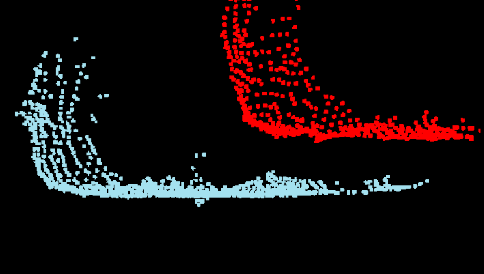
\includegraphics[height=.28\linewidth]{icp-init}
  }
  \subfigure[Stuck in a local maximum after 3 iterations
  (green arrows)]{%
    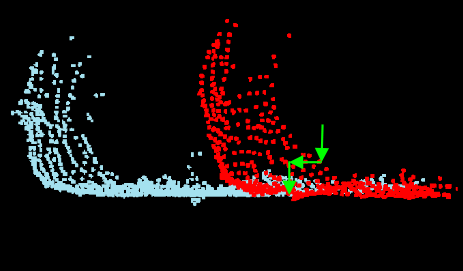
\includegraphics[height=.28\linewidth]{icp-stuck}
  }
  
  \caption{Possible case for bad ICP alignment results. The two point
    clouds belong a detected car in successive frames~\cite{held-website}.}
  \label{fig:icp}
\end{figure}
The approach presented in this report performs a global search and
therefore has no problem with local maxima.

\subsection{Alternative Sensors}
\label{sub:slternative-sensors}
Laser range sensors, such as the one shown in Figure~\ref{fig:lidar},
are not the only kind of sensors used for tracking tasks. Although
laser range sensors provide more precise data compared to other
sensors used for tracking, they are inadequate
for many applications because of their high price. the closest
alternative to laser range sensors is the usage of stereo
cameras. They provide the same kind of data (point clouds and images)
and are cheap. However, they have more noise then a laser sensor and
can therefore cause larger errors in the tracing results. An example
for the use of stereo data for tracking
is~\cite{leibe-tracking-before-detection}. It uses ICP to track
pedestrians and unknown objects. Object tracking with a single camera
has been studied for a long time and is used in many applications,
e.g. in video calling~\cite{single-camera-tracking}. However, single
camera tracking is unsuitable in the autonomous car scenario because
of missing depth information.

\subsection{Grid-Based Methods}
\label{sub:grid-based-methods}
Ordinary grid-based search approaches in computer vision are used to
globally search in a state space and allow multiple hypothesis in
contrast to Kalman filters and ICP. However, the computationally
effort increases with the resolution of the grid and therefore
ordinary histograms are often inadequate for real time computation.
Dynamic histograms tackle this problem by starting with a low
resolution and increasing the resolution in important areas. However,
this creates the problem that the low resolution introduces an
additional error.

There are some alternative grid-based approaches to annealed dynamic
histograms. Most of them are used in Simultaneous Localization and
Mapping (\textit{SLAM}). \cite{multi-res-grid-slam2} uses a grid-based
Monte-Carlo method that recursively expands the grid cells with the
most hypotheses and refines the grid resolution in these cells. This
only differs from annealed dynamic histograms in the usage of a
Monte-Carlo distribution instead of probabilities to cause the current
measurement. The approach presented in~\cite{multi-res-grid-slam}
self-localizes a robot with a dynamically refined grid. Here each
measurement point votes for the cells that could have caused the
measurement. The cells with the most votes are refined in the next
iteration. Similarly to the paper presented in this report, the
approach enables anytime computation.

The main differences between previous methods and the method presented
in this report are the additional consideration of color, what is not
directly possible in Kalman filter or ICP approaches, and the
consideration of the probabilities for points being occluded in
previous frames. This leads to higher tracking
robustness. Furthermore, annealed dynamic histograms allow globally
searching the state space, multiple hypotheses. In contrast to other
grid-based approaches, it also allows real-time computation without
introducing a high error resulting from low resolution by
annealing the measurement model as the resolution increases.

% +++++++++++++++++++++++++
\section{Method}
\label{sec:method}
The method presented in this report consists of three major
parts. Subsection~\ref{sub:probabilistic-model} introduces the
probabilistic model based on a Dynamic Bayesian Network. The model is
necessary to determine how likely it is that a specific position and
velocity of a detected object causes the observed
measurement. Subsection~\ref{sub:adh} describes how annealed dynamic
histograms are used to search the state space for the most likely
position and velocity according to the measurement model. For that
especially the refinement steps, that increase the resolution, and the
annealing of the measurement model depending on the resolution are
important. In Subsection~\ref{sub:adding-color} the extension of the
measurement model by color is shown~\cite{paper}.

\subsection{Probabilistic Model}
\label{sub:probabilistic-model}

\begin{figure}
  \center
  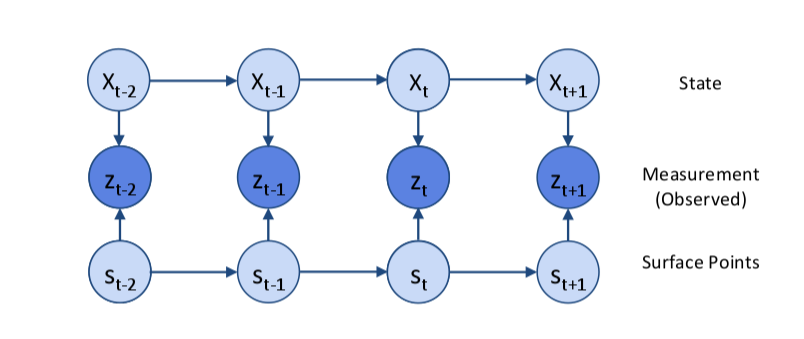
\includegraphics[width=.8\linewidth]{dbn}
  \caption{Dynamic Bayesian Network to model the measurement for
    tracking an object~\cite{paper}.}
  \label{fig:dbn}
\end{figure}

To derive the probability for a position and velocity to cause the
observed measurement seen in the last frames, we use a Bayesian
Network because it allows us to easily combine 3D shape, color, and
motion in the model. After encoding the influences of the states,
consisting of position and velocity, the surface of the object to
track and the observed measurement, we can derive the wanted
probability of the measurement given the state by applying well known
probability rules in Bayesian Networks~\cite{ai-modern}. Furthermore
we use a Dynamic Bayesian Network to relate variables over successive
time steps.

The Dynamic Bayesian Network we use to derive the measurement model is
shown in Figure~\ref{fig:dbn}. For the frames $t-2$ to the current
frame $t+1$, it includes the variables $x$ for the state, $z$ for the
observed measurement and $s$ for the visible surface of the object. In
the following we describe these variables in detail.

As state variable $x_t$, we use the composition of position and
velocity $x_t=(x_{t,p},\dot{x}_{t,p})$. $x_{t,p}$ is the linear
position of the object centroid in frame $t$ relative to the centroid
of the object in frame $t-1$. In other words, the centroid of the
object in frame $t-1$ is the origin of the coordinate system for
$x_{t,p}$. $\dot{x}_{t,p}$ is the velocity of the object. The relative
rotation and the rotational velocity of the object is not included in
the state. This speeds up the method because a lower dimensional state
space is considered. The authors claim that omitting the rotation is
no problem because the rotational velocity of the objects present in
traffic is small relative to the frame rate of the sensor, which is
$10Hz$. Similarly, also the vertical movement of the objects is very
small because the objects we are interested in move along the
ground. Therefore, we can use a 2D position and velocity instead of a
3D position and velocity. To use the methods in other domains that
require considering the vertical velocity, the state space can be
expanded, what results in a slow down of the method.
%Alternative elivation map?

To include the 3D shape of the object in the model we use the latent
surface variable $s_t$. It represents the visible surface of the
object and is a set of $n$ points $\{s_{t,1}, ..., s_{t,n}\} = s_t$
that are sampled from the visible surface. Although the true 3D shape
of the object is unknown and only indirectly observable through the
measurement it is important for the model. This is similar to SLAM
methods which model the environment map, the surface in our
terminology. The measurement then depends on the modeled map and the
localization, or the object surface and state in our case. When
looking at the Dynamic Bayesian Network in Figure~\ref{fig:dbn}, it is
easy to see that considering the surface is important because, when it
is omitted, two successive measurements would be independent given the
state variable. This would be wrong because the shape of the object is
relatively consistent and therefore also the measurement points
describe a similar surface. In contrast to SLAM, it is not our goal to
build the shape of the observed object. We simply integrate over
shapes to get the surface. The prior of the surface points
$p(s_{t,i})$ is a uniform distribution over the maximum size of an
object. The prior of the surface is the product over its points
$p(s_{t})=\Pi_i p(s_{t,i})$.

\begin{wrapfigure}{r}{0.45\linewidth}
  \center
  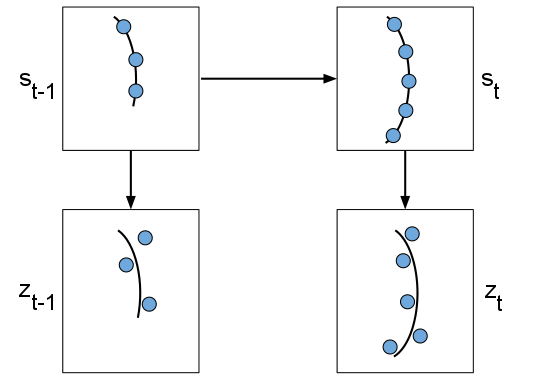
\includegraphics[width=\linewidth]{surface-measurement}
  \caption{Measurement points $z_t$ sampled with sensor noise
    $\Sigma_e$ from surface points $s_t$. The visible surface, from which the
    surface points are sampled, varies from frame to frame due to
    occlusion and viewpoint changes~\cite{paper}.}
  \label{fig:surface-measurement}
\end{wrapfigure}

The observed measurement $z_t$ is again a set of measurement points
$z_t=\{z_{t,1}, ..., z_{t,m}\}$. These points depend on the latent
surface $s_t$ and the position $x_{t,p}$. However, the measurement
points do not lie directly on the surface as illustrated in
Figure~\ref{fig:surface-measurement}. This is caused by the sensor
noise, which depends on the sensor resolution and is modeled as
Gaussian noise $\Sigma_e$. The sensor resolution can be modeled as a
roughly linear function of the distance between object and sensor. The
generation of measurement points $z_t$ depending on the surface points
$s_t$, the sensor noise $\Sigma_e$ and the position can be written as
\begin{equation}
\label{eq:gaus-zt}
z_{t,i} \sim \mathcal{N}(s_{t,i},\Sigma_e) + x_{t,p} \mbox{ . }
\end{equation}
Because the origin of the coordinate system is placed at the centroid
of the object in the previous frame, the measurements of the previous
frame are not shifted
\begin{equation}
\label{eq:ind-centroid}
z_{t-1,i} \sim \mathcal{N}(s_{t-1,i},\Sigma_e) \mbox{ . }
\end{equation}
Therefore $z_{t-1}$ is conditionally independent from $x_{t-1}$ what
is not derivable by just using the Bayesian Network in
Figure~\ref{fig:dbn}.

For the derivation of the measurement model, we will also need the
term $p(s_t|s_{t-1})$ which stands for the probability of sampling
surface points $s_t$ from the currently visible surface given
$s_{t-1}$ from the previous frame. The sampled points might differ
because of occlusions, viewpoint changes, random sampling from the
surface and deformations of the object (e.g. body movement of a
walking pedestrian). Every point of $s_t$ could have been generated
from a visible or occluded part of the surface in frame $t-1$. When we
consider the prior probability $p(V)$ for sampling from a previously
visible surface, we can use the joint distribution over these two
cases:
\begin{equation}
\label{eq:st-st-1}
p(s_{t,i}|s_{t-1})=p(V)*p(s_{t,i}|s_{t-1},V) + p(\neg V)*p(s_{t,i}|s_{t-1},\neg V)
\end{equation}
$p(s_{t,i}|s_{t-1},\neg V)$ stands for the probability that $s_{t,i}$
is generated from a part of the surface that was not visible in the
previous frame. Under the assumption that every non visible point is
occluded, we can rewrite the term with constants $k_1$ and $k_2$:
\begin{equation}
p(s_{t,i}|s_{t-1},\neg V) = k_1 (k_2 - p(s_{t,i}|s_{t-1},V))
\end{equation}
This allows simplifying Equation~\ref{eq:st-st-1} to
\begin{equation}
\label{eq:prob-surf}
p(s_{t,i}|s_{t-1})=\eta_1 (p(s_{t,i}|s_{t-1},V) + k)
\end{equation}
with the normalization constant $\eta_1=p(V)-p(\neg V) k_1$ and the
smoothing factor $k=p(\neg V)k_1k_2/\eta_1$.
%Possible equation
These constants can later be found by training.

$p(s_{t,i}|s_{t-1},V)$ can be modeled by a
Gaussian distribution
\begin{equation}
\label{eq:gaus-st-i}
s_{t,i} \sim \mathcal{N}(s_{t-1,i},\Sigma_r)
\end{equation}
where $s_{t-1,i}$ is the closest corresponding surface point from the
previous frame and $\Sigma_r$ is the variance mainly resulting from
the sensor resolution and the object deformation. Combining these
Gaussians in Equation~\ref{eq:prob-surf} for all surface points in
$s_t$ yields
\begin{equation}
\label{eq:gaus-st}
p(s_{t}|s_{t-1}) = \eta(\mathcal{N}(s_t;s_{t-1,i},\Sigma_r) + k) \mathrm{ . }
\end{equation}

For the measurement model used in the annealed dynamic histogram, we
need to derive $p(z_t|x_t,z_1,...,z_{t-1})$, the probability for the
current measurement given the histogram cell with state $x_t$ and the
previous measurements $z_1$ to $z_{t-1}$. Though considering all
previous measurements of the object would be computationally
costly. Although the measurements in different time frames are not
independent given the state, as discussed earlier, we can focus only
on the previous one as approximation, because the previous one has the
highest impact of all measurements in the history.
\begin{equation}
p(z_t|x_t,z_1,...,z_{t-1}) \approx p(z_t|x_t,z_{t-1})
\end{equation}
This approximation can be rewritten by using the joint distribution over
all surface points in the current and previous frame:
\begin{equation}
\label{eq:mm-iint}
p(z_t|x_t,z_{t-1}) = \iint p(z_t,s_t,s_{t-1}|x_t,z_{t-1}) \mathrm d
s_t \mathrm d s_{t-1}
\end{equation}
Because of the chain rule of probabilities and the conditional
independences that could be derived from the Dynamic Bayesian Network
in Figure~\ref{fig:dbn} we can refine the term in the integral:
\begin{align}
p(z_t,s_t,s_{t-1}|x_t,z_{t-1})
&= p(z_t|s_t,x_t)p(s_t|s_{t-1})p(s_{t-1}|x_t,z_{t-1})\nonumber\\
&\overset{(\ref{eq:ind-centroid})}{=} p(z_t|s_t,x_t)p(s_t|s_{t-1})p(s_{t-1}|z_{t-1})\nonumber\\
&= \eta_2p(z_t|s_t,x_t)p(s_t|s_{t-1})p(z_{t-1}|s_{t-1})p(s_{t-1})
\end{align}
$\eta_2$ is again a normalization constant and can be used to absorb
the constant term $p(s_{t-1})$. This term is constant because it is
the product of a constant number of uniformly distributed
probabilities of the surface points. This allows simplifying the
term in the integral further:
\begin{align}
\label{eq:meas-mod-before-convolution}
p(z_t,s_t,s_{t-1}|x_t,z_{t-1})
&=\eta\underbrace{p(z_t|s_t,x_t)}_{(\ref{eq:gaus-zt})}\underbrace{p(s_t|s_{t-1})}_{(\ref{eq:gaus-st})}\underbrace{p(z_{t-1}|s_{t-1})}_{(\ref{eq:ind-centroid})}
\end{align}
For this term, we have modeled all probabilities as Gaussians as
indicated under Equation~\ref{eq:meas-mod-before-convolution}.
Therefore, the term only consists of a product of Gaussians and
Gaussians plus a constant. If we plug in
Equation~\ref{eq:meas-mod-before-convolution} back into our integrals
in Equation~\ref{eq:mm-iint}, we can apply a convolution of Gaussians
to solve the inner integral~\cite{prob-rob}. Because the convolution of two Gaussians
results in a Gaussian, we can apply a convolution of Gaussians again
to evaluate the outer integral and yield a Gaussian for the
measurement model:
\begin{equation}
\label{eq:gaus-mm}
p(z_t|x_t,z_{t-1}) =
\eta(\mathcal{N}(z_t;z_{t-1}+x_{t,p},\Sigma_r+2\Sigma_e)+k)
\end{equation}
For the computation of the measurement model, we introduce the
variable $\bar{z}_{t-1}=z_{t-1}+x_{t,p}$ so that the measurement in
the previous frame is shifted according to $x_t$. Then for each
$z_{t,i}\in z_t$, we have to find the closest corresponding point
$\mathrm{ccp}(z_{t,i}) = \bar{z}_{t-1,j}\in \bar{z}_{t-1}$. The measurement
probability for the current measurement given the inspected state and
the previous measurements can be computed by
\begin{equation}
\label{eq:gaus-mm}
p(z_t|x_t,z_{t-1}) =
\eta\left(\prod_{z_{t,i}\in z_t}
\mathrm{exp}\left(-\frac{1}{2}(z_{t,i}-\mathrm{ccp}(z_{t,i}))^T\Sigma^{-1}(z_{t,i}-\mathrm{ccp}(z_{t,i}))\right)+k\right)
\end{equation}
with normalization constant $\eta$, smoothing factor $k$, and
covariance matrix $\Sigma = 2\Sigma_e+\Sigma_r$. Again these constants
and the function for $\Sigma_r$ depending on the distance between
sensor and tracked object can be found by optimizing for a set of
training data.

\subsection{Adding Color and Motion}
\label{sub:adding-color}
\subsection{Annealed Dynamic Histograms}
\label{sub:adh}

% +++++++++++++++++++++++++
\section{Evaluation}
\label{sec:evaluation}
\subsection{Relative Reference Frame}
\label{sub:relative-ref-frame}
\subsection{Model Crispness}
\label{sub:model-crispness}

% +++++++++++++++++++++++++
\section{Conclusion}
\label{sec:conclusion}


% =========================================================================
\bibliographystyle{alpha}
\bibliography{seminar_report}

% =========================================================================

\end{document}
